\chapter{Introduction}
  \section{Généralités}

Le projet Link-Pix s'inscrit dans le cadre de l'UE GLIN405 proposée au semestre 4 du parcours Informatique.
L'objectif de ce projet est la mise en place d'un travail de groupe pour la conception et la réalisation d'un projet informatique.
L'organisation, la distribution du travail, la communication sont des éléments essentiels à la réussite du projet, et apporteront aux participants un savoir-faire pratique du travail de groupe.

Le projet devra être fini aux dates de soutenance, c'est à dire les 30 et 31 mai 2013.

Le groupe pour le projet Link-Pix se compose de six membres, une répartition du travail devra par conséquent être faite.

Chaque groupe est encadré par un tuteur, Philippe Janssen dans notre cas, chargé d'encadrer et de guider le groupe.

  \section{Le sujet}

L'objectif de ce projet est la réalisation d'un solveur pour les puzzles de type Link-Pix, dont les détails seront donnés ci-dessous.

    \subsection{Principe du Link-Pix}
Les puzzles de type Link-Pix (aussi connus sous le nom de Link-a-Pix) sont des puzzles images. Le puzzle est une grille rectangulaire dont certaines cases (appelées indice par la suite) contiennent des nombres positifs.

La résolution du puzzle fait apparaître une image, sous la forme d'une grille de même taille dont chaque case est soit noire, soit blanche.

Cette image est obtenue en reliant par un chemin, comprenant les indices, chaque couple d'indices selon les contraintes suivantes :
\begin{itemize}
    \item un indice de valeur 1 est lié à lui-même~;
    \item un indice ne peut être relié qu'à un seul autre indice de même valeur~;
    \item deux indices de valeur $n$ doivent être reliés par un chemin de $n$ cases~;
    \item deux chemins ne peuvent pas se croiser~;
    \item un chemin ne peut pas se recouper.
\end{itemize}
Ainsi, deux cases d'indice 3 devront être reliées avec un chemin de longueur 3.
\begin{figure}[h]
      \centering
      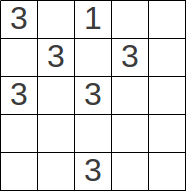
\includegraphics[scale=0.5]{puzzle01}
      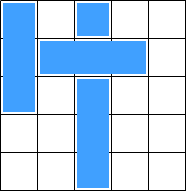
\includegraphics[scale=0.5]{puzzle01-sol}
      \caption{Exemple de puzzle $5 \times 5$ de type Link-Pix et son unique solution.}
\end{figure}

    \subsection{Sujet}
    L'objectif du projet se divise en deux parties :
    \begin{itemize}
    \item la première partie est la création d'un solveur, un programme capable d'analyser une grille et de rendre l'image résultat~;
    \item la seconde partie est l'analyse d'une image dans l'objectif de créer une grille correspondant à cette image.
    \end{itemize}
    Ainsi, le programme final devra être capable de résoudre des puzzles de type Link-Pix, dévoilant l'image cachée par le problème.

  \section{Cahier des charges}

  \subsection{Fonctionnalités}
Le solveur devra, à partir d'un puzzle, analyser la grille et trouver la solution de celle-ci.

L'analyseur devra quant à lui être capable, à partir d'une image donnée, d'analyser cette image et de renvoyer une grille de type Link-Pix qui possède une unique solution.

  \subsection{Contraintes}
  Le solveur doit être capable de lire une grille enregistrée dans un fichier, selon un format défini, afin de l'analyser.

  Il a été décidé que le solveur ne traiterait que le cas des puzzles à solution unique, ceci afin de faciliter le développement.

  Il doit également se composer d'une interface graphique permettant de suivre l'évolution pas à pas de la résolution.

  En outre, le développement de la seconde partie, l'analyse de l'image et la création d'une grille correspondante, a été abandonné quasiment dès le début. Ceci est principalement dû au désistement de certains membres du groupe, ne nous permettant pas de travailler parallèlement sur les deux parties. La partie solveur a ainsi été privilégiée.
